\documentclass[11pt]{article}
\usepackage[T1]{fontenc}
\usepackage[utf8]{inputenc}
\usepackage{lmodern,amsmath,amssymb,graphicx,geometry,microtype,setspace,booktabs,caption}
\usepackage[hidelinks]{hyperref}
\geometry{letterpaper,margin=1in}
\setlength{\parindent}{0pt}
\setlength{\parskip}{0.55em}
\setlength{\emergencystretch}{2em}
\captionsetup{labelfont=bf,font=small}
\renewcommand{\refname}{References}

\pagestyle{empty}
\renewcommand{\thefigure}{S\arabic{figure}}
\setcounter{figure}{7}

\begin{document}
\begin{figure}[!ht]\centering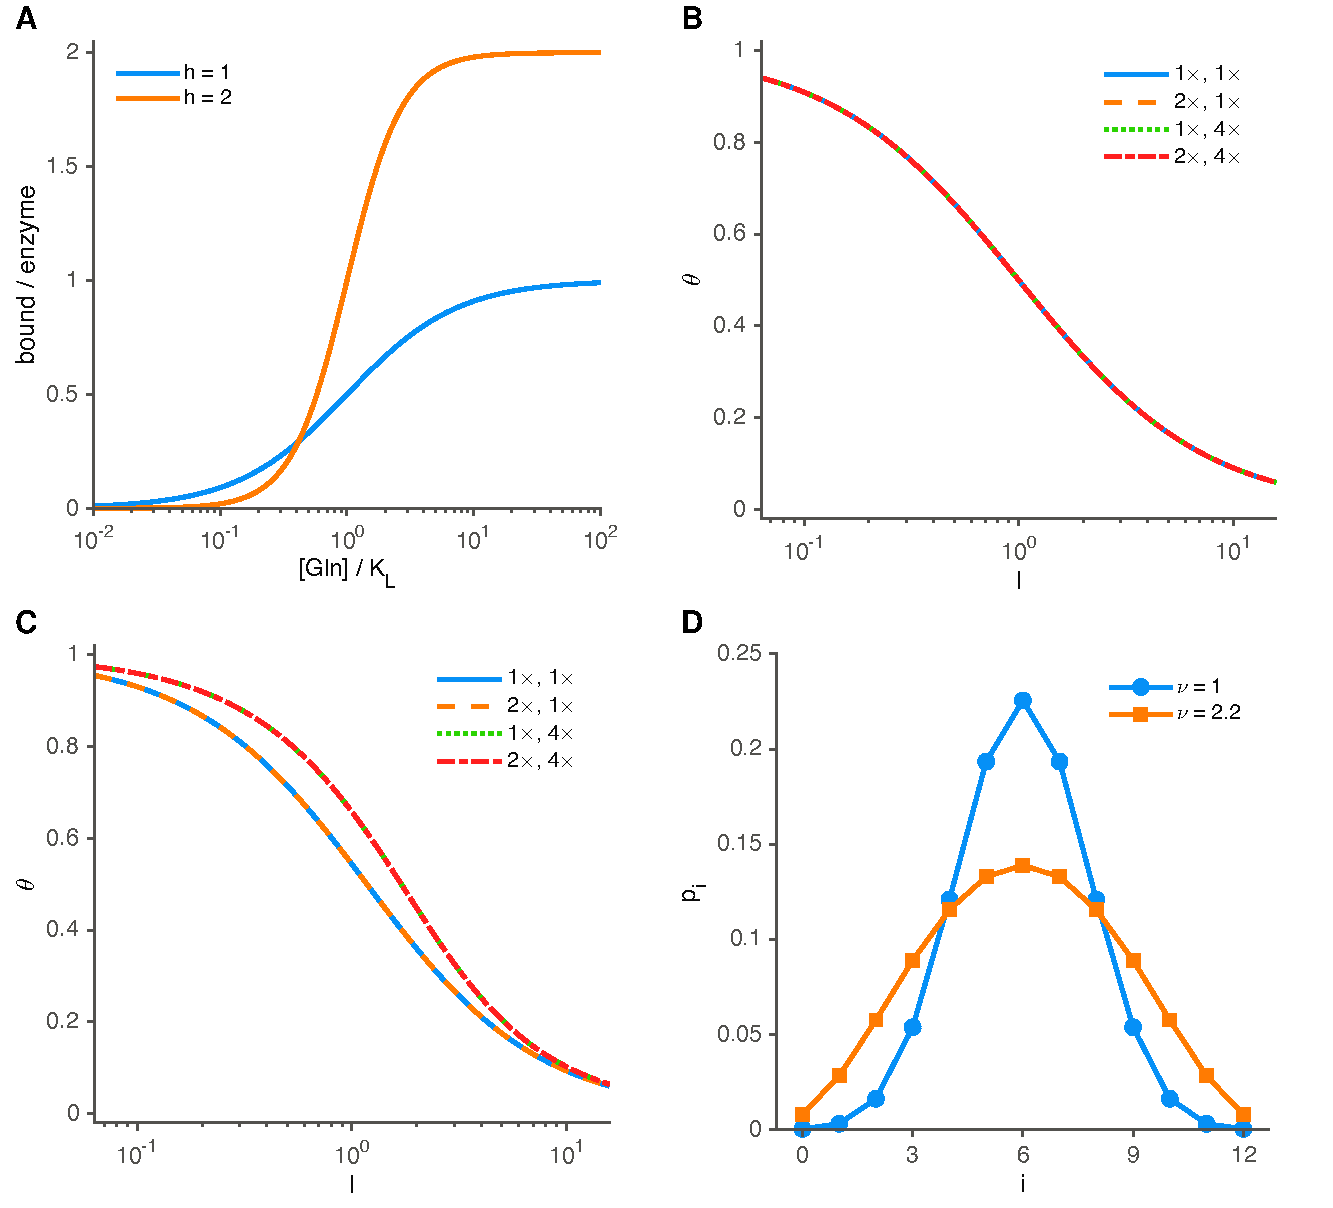
\includegraphics[width=\textwidth,height=0.62\textheight,keepaspectratio]{figure_inputs/FigS8_design.pdf}\begin{singlespace}\caption{\textbf{Measurements that discriminate unresolved mechanisms.} (A) Illustrative one-ligand and concerted two-ligand binding laws, expressed as ligands per enzyme. Activity measurements must accompany occupancy to identify productive states. (B) Illustrative minimal-model total-target responses at two enzyme and two target levels. Parameters are n=3, A=1, $\widehat B$=Ghat=0.4, $\widehat K$=1, baseline $T_E$=0.0001 and $T_S$=1 in consistent concentration units; the four curves nearly coincide because the enzyme pool is dilute. (C) An illustrative active target-bridging extension with one modification site and relation s\_1=$s_0$/(l-0.35$s_0$), with total free target 1 or 4. Target levels separate; enzyme levels coincide in this reduced construction. These examples are not fits to the measured titration. (D) Twelve-site distributions with the same mean modification but $\nu$=1 or $\nu$=2.2, generated by exponential reweighting of binomial states as specified in S1 Appendix. These distributions are not fits to glutamine synthetase.}\end{singlespace}\end{figure}
\end{document}
